\documentclass[UTF8]{article}
\usepackage{CTEX}
\usepackage{graphicx, subfig}
\usepackage{float}
\begin{document}

这是一个CTEX的utf-8编码例子,{\kaishu 这里是楷体显示},{\songti 这里是宋体显示},{\heiti 这里是黑体显示},{\fangsong 这里是仿宋显示},{\lishu 这里是隶书显示},{\youyuan 这里是幼圆显示}。

如图,设双曲线$C$:$\frac{x^2}{a^2}-\frac{y^2}{b^2}=1(a>0,b>0)$的左右顶点分别为$A$、$B$,已知双曲线的焦距等于实轴长的2倍,虚轴长为$2\sqrt{3}$ 。

(1)求双曲线$C$的方程;

(2)设$Q$为双曲线$C$上异于$A$,$B$的点,求证:直线$QA$与$QB$的斜率之积为定值;

(3)若直线$l:y=x+m$与双曲线$C$交于$D$、$E$两点,试探究是否存在实数$m$,使得$|AD|=|AE|$?若存在,求出$m$的值;若不存在,说明理由。

\begin{figure}[H]
  \centering
  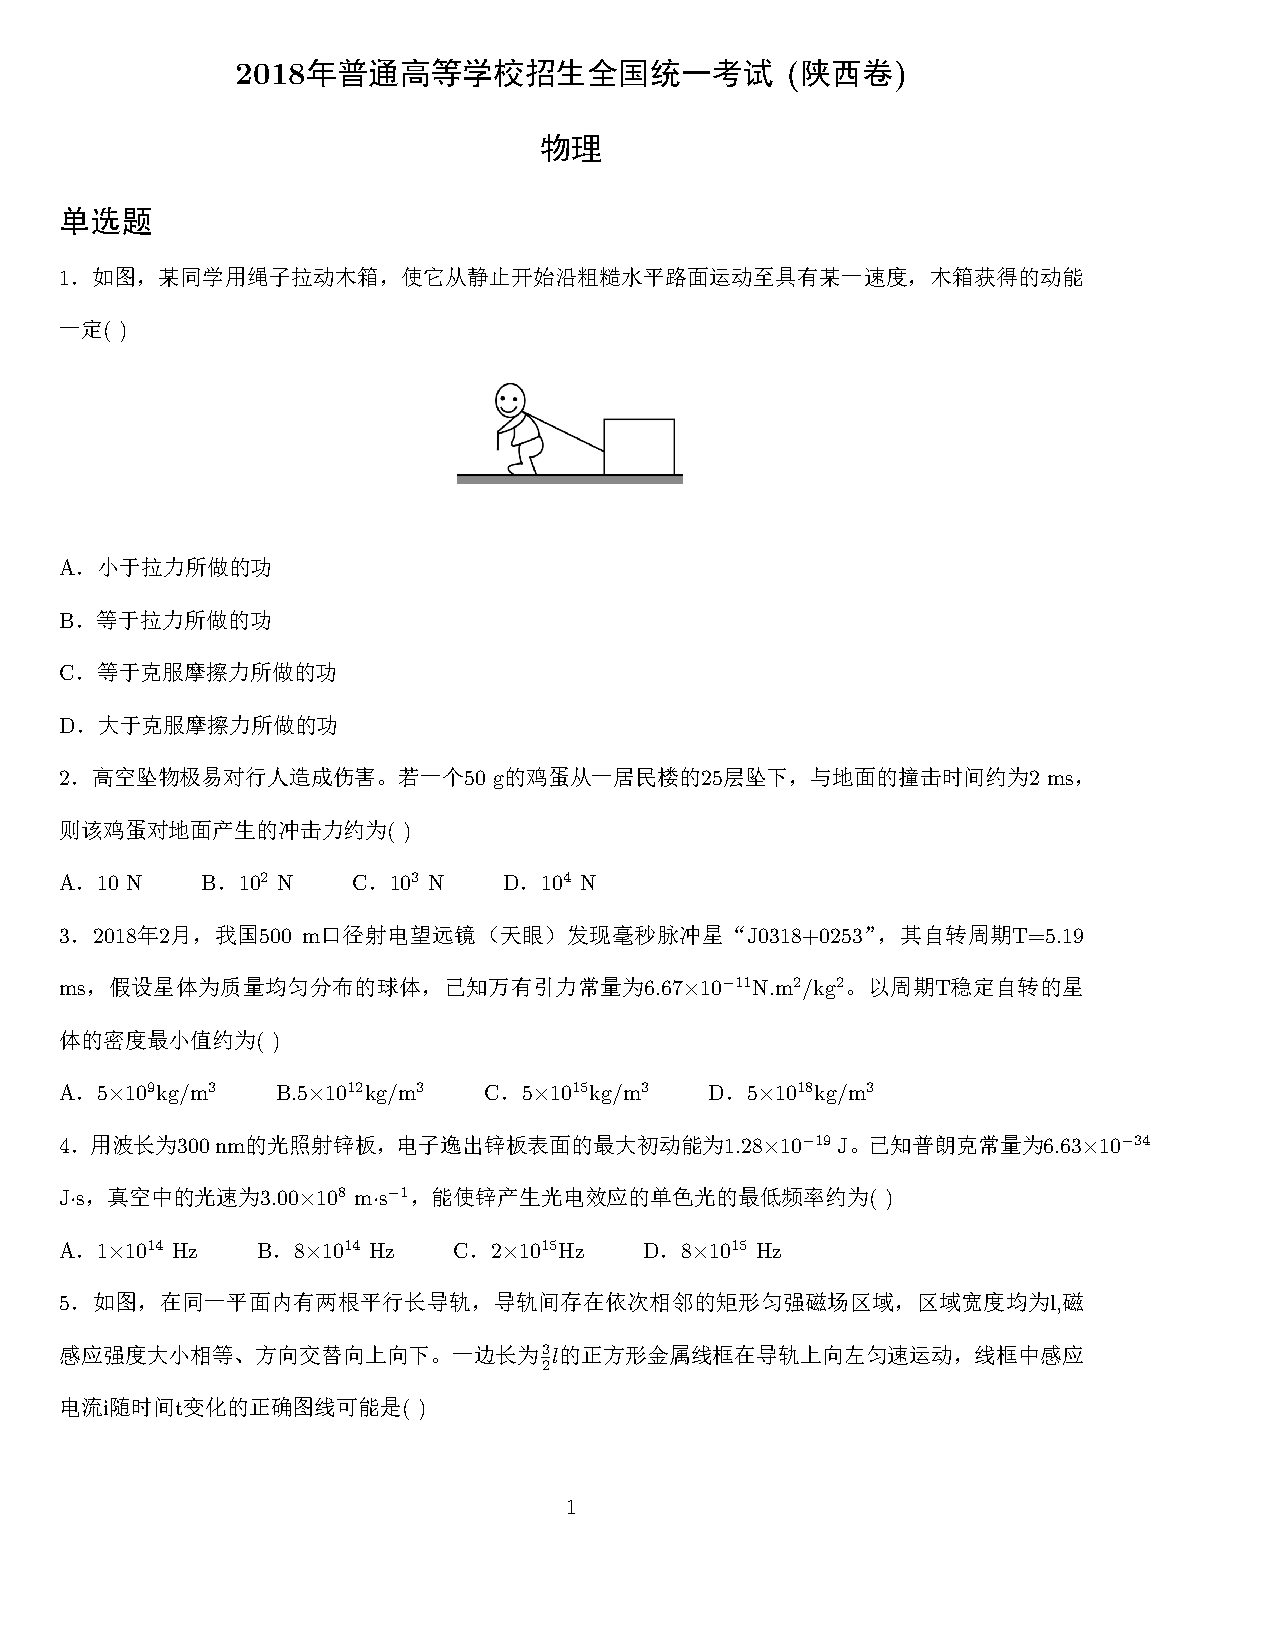
\includegraphics[width=.5\textwidth]{C:/Users/吴青峰/PycharmProjects/math_to_csv/test.png} %1.png是图片文件的相对路径
  \caption{best} %caption是图片的标题
 \end{figure}
 
\end{document}